\documentclass[11pt]{article}

% =========================
% Packages
% =========================
\usepackage[margin=0.78in]{geometry}
\usepackage{amsmath,amssymb,amsfonts,mathtools}
\usepackage{booktabs,array,tabularx,longtable,multirow}
\usepackage{enumitem}
\usepackage[most]{tcolorbox}
\usepackage{xcolor}
\usepackage{fancyhdr}
\usepackage{titlesec}
\usepackage{hyperref}
\usepackage{lastpage}
\usepackage{setspace}
\usepackage{tikz}
\usepackage{pgfplots}
\usepackage{needspace}
\usepackage{caption}
\usepackage{multicol}
\usepackage{graphicx}
\usepackage{amsthm}
\usepackage{mathrsfs}
\usepackage{bm}
\usepackage{float}
\usepackage{changepage}
\usetikzlibrary{calc,arrows.meta,positioning,decorations.pathreplacing,patterns,angles,quotes}

\pgfplotsset{compat=1.18}
\setstretch{1.14}
\setlength{\parindent}{0pt}
\setlength{\parskip}{0.45em}
\setlist[itemize]{leftmargin=1.8em}
\setlist[enumerate]{leftmargin=2em}

% =========================
% Colors
% =========================
\definecolor{novelPurple}{RGB}{98,54,255}
\definecolor{novelPurpleDark}{RGB}{72,34,204}
\definecolor{novelPurpleLight}{RGB}{243,239,255}
\definecolor{novelPurpleLine}{RGB}{165,135,255}
\definecolor{npgray}{RGB}{78,78,78}
\definecolor{softgray}{RGB}{246,246,250}
\definecolor{softlav}{RGB}{249,247,255}
\definecolor{greencheck}{RGB}{24,128,88}
\definecolor{warmred}{RGB}{188,54,54}
\definecolor{nporange}{RGB}{223,121,36}
\definecolor{npgreen}{RGB}{67,142,103}
\definecolor{npred}{RGB}{180,54,54}

% =========================
% Hyperref
% =========================
\hypersetup{
    colorlinks=true,
    linkcolor=novelPurpleDark,
    urlcolor=novelPurpleDark,
    citecolor=novelPurpleDark
}

% =========================
% Header / Footer
% =========================
\pagestyle{fancy}
\fancyhf{}
\fancyhead[L]{\textbf{Novel Prep Learning Center}}
\fancyhead[R]{\textbf{AP Calculus AB --- Unit 4}}
\fancyfoot[C]{\textcolor{novelPurpleDark}{\thepage\ /\ \pageref{LastPage}}}
\renewcommand{\headrulewidth}{0.4pt}
\renewcommand{\footrulewidth}{0pt}

% =========================
% Section styles
% =========================
\setcounter{secnumdepth}{3}
\setcounter{tocdepth}{3}

\titleformat{\section}
{\Large\bfseries\color{novelPurpleDark}}{\thesection.}{0.6em}{}

\titleformat{\subsection}
{\large\bfseries\color{novelPurple}}{\thesubsection.}{0.6em}{}

\titleformat{\subsubsection}
{\normalsize\bfseries\color{novelPurpleDark}}{\thesubsubsection.}{0.6em}{}

% =========================
% Boxes
% =========================
\tcbset{enhanced,sharp corners,boxrule=1pt}

\newtcolorbox{theorybox}[1]{
  colback=white,
  colframe=novelPurple,
  colbacktitle=novelPurple,
  coltitle=white,
  title=\textbf{#1},
  fonttitle=\bfseries,
  sharp corners,
  breakable
}

\newtcolorbox{notebox}[1]{
  colback=novelPurpleLight,
  colframe=novelPurple,
  colbacktitle=novelPurple,
  coltitle=white,
  title=\textbf{#1},
  fonttitle=\bfseries,
  sharp corners,
  breakable
}

\newtcolorbox{skillbox}[1]{
  colback=softlav,
  colframe=novelPurpleDark,
  colbacktitle=novelPurpleDark,
  coltitle=white,
  title=\textbf{#1},
  fonttitle=\bfseries,
  sharp corners,
  breakable
}

\newtcolorbox{summarybox}[1]{
  colback=softgray,
  colframe=novelPurpleDark,
  colbacktitle=novelPurpleDark,
  coltitle=white,
  title=\textbf{#1},
  fonttitle=\bfseries,
  sharp corners,
  breakable
}

\newtcolorbox{practicebox}[1]{
  colback=white,
  colframe=novelPurpleLine,
  colbacktitle=novelPurpleLine,
  coltitle=black,
  title=\textbf{#1},
  fonttitle=\bfseries,
  sharp corners,
  breakable
}

% =========================
% Commands
% =========================
\newcounter{examplectr}[subsection]
\renewcommand{\theexamplectr}{\thesubsection.\arabic{examplectr}}

\newcommand{\example}[1]{%
\refstepcounter{examplectr}
\Needspace{8\baselineskip}
\noindent{\color{novelPurpleDark}\textbf{Example \theexamplectr.}} \textbf{#1}\par
}

\newcommand{\solution}{\noindent{\textbf{Solution.}}}
\newcommand{\unitchapter}[1]{\newpage\subsection{#1}}
\newcommand{\unitsubtopic}[1]{\subsubsection{#1}}

% =========================
% Figures
% =========================
\newcommand{\unitfourcoverfigure}{
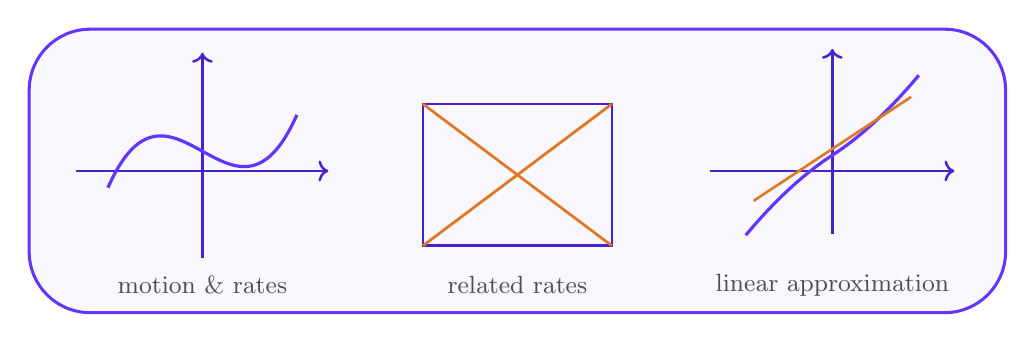
\begin{tikzpicture}[scale=1]
\fill[softlav,rounded corners=22pt] (-6.2,-1.8) rectangle (6.2,1.8);
\draw[novelPurple, line width=1.1pt, rounded corners=22pt] (-6.2,-1.8) rectangle (6.2,1.8);

\begin{scope}[shift={(-4.0,0)}]
\draw[novelPurpleDark, line width=0.9pt, ->] (-1.6,0)--(1.6,0);
\draw[novelPurpleDark, line width=0.9pt, ->] (0,-1.1)--(0,1.5);
\draw[novelPurple, line width=1.15pt, smooth, samples=160, domain=-1.2:1.2]
plot (\x,{0.65*\x^3-0.55*\x+0.25});
\node[text=npgray] at (0,-1.45) {\small motion \& rates};
\end{scope}

\begin{scope}[shift={(0,0)}]
\draw[novelPurpleDark, line width=0.9pt] (-1.2,-0.95)--(1.2,-0.95)--(1.2,0.85)--(-1.2,0.85)--cycle;
\draw[nporange, line width=1.0pt] (-1.2,-0.95)--(1.2,0.85);
\draw[nporange, line width=1.0pt] (-1.2,0.85)--(1.2,-0.95);
\node[text=npgray] at (0,-1.45) {\small related rates};
\end{scope}

\begin{scope}[shift={(4.0,0)}]
\draw[novelPurpleDark, line width=0.9pt, ->] (-1.55,0)--(1.55,0);
\draw[novelPurpleDark, line width=0.9pt, ->] (0,-0.8)--(0,1.55);
\draw[novelPurple, line width=1.15pt, smooth, domain=-1.1:1.1, samples=160]
plot (\x,{0.25*\x^2+0.65*\x+0.2});
\draw[nporange, line width=0.95pt] (-1.0,-0.38)--(1.0,0.94);
\node[text=npgray] at (0,-1.45) {\small linear approximation};
\end{scope}

;
\end{tikzpicture}
}

\newcommand{\unitsfigure}{
\begin{center}
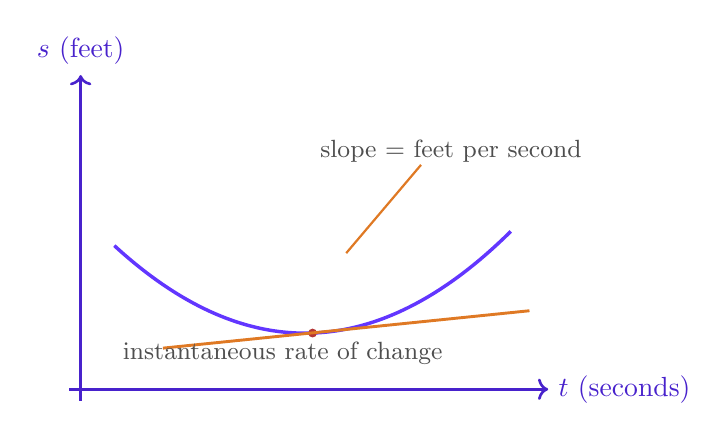
\begin{tikzpicture}[x=0.95cm,y=0.95cm]
    % axes
    \draw[novelPurpleDark, line width=0.95pt, ->] (-0.15,0) -- (6.25,0) node[right] {$t$ (seconds)};
    \draw[novelPurpleDark, line width=0.95pt, ->] (0,-0.15) -- (0,4.2) node[above] {$s$ (feet)};

    % position curve
    \draw[novelPurple, line width=1.25pt, smooth, samples=220, domain=0.45:5.75]
        plot (\x,{0.18*(\x-3.0)^2 + 0.75});

    % point of tangency
    \pgfmathsetmacro{\xc}{3.1}
    \pgfmathsetmacro{\yc}{0.18*(\xc-3.0)^2 + 0.75}
    \fill[npred] (\xc,\yc) circle (1.6pt);

    % tangent line
    \draw[nporange, line width=1.05pt] (1.1,0.55) -- (6,1.05);

    % pointer to tangent
    \draw[nporange, line width=0.8pt] (4.55,3.0) -- (3.55,1.82);
    \node[text=npgray] at (4.95,3.18) {\small slope = feet per second};

    % local label
    \node[text=npgray] at (2.7,0.48) {\small instantaneous rate of change};
\end{tikzpicture}
\end{center}
}

\newcommand{\motionoverviewfigure}{
\begin{center}
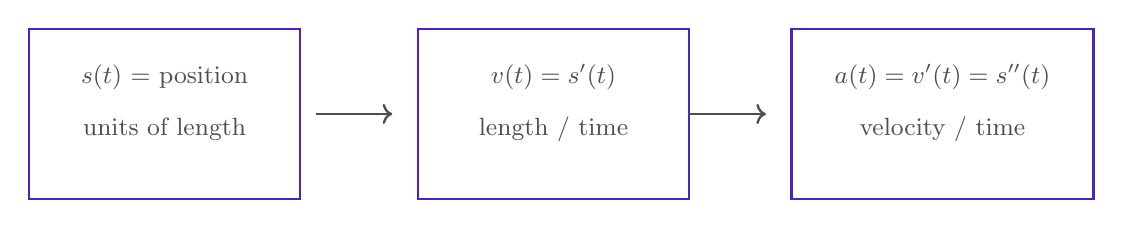
\begin{tikzpicture}[x=1.3cm,y=0.9cm]
    \begin{scope}[shift={(0,0)}]
        \draw[novelPurpleDark, line width=0.9pt] (0,0) rectangle (2.65,2.4);
        \node[text=npgray] at (1.325,1.72) {\small $s(t)$ = position};
        \node[text=npgray] at (1.325,0.98) {\small units of length};
    \end{scope}

    \draw[->, line width=0.85pt, npgray] (2.8,1.2)--(3.55,1.2);

    \begin{scope}[shift={(3.8,0)}]
        \draw[novelPurpleDark, line width=0.9pt] (0,0) rectangle (2.65,2.4);
        \node[text=npgray] at (1.325,1.72) {\small $v(t)=s'(t)$};
        \node[text=npgray] at (1.325,0.98) {\small length / time};
    \end{scope}

    \draw[->, line width=0.85pt, npgray] (6.45,1.2)--(7.2,1.2);

    \begin{scope}[shift={(7.45,0)}]
        \draw[novelPurpleDark, line width=0.9pt] (0,0) rectangle (2.95,2.4);
        \node[text=npgray] at (1.475,1.72) {\small $a(t)=v'(t)=s''(t)$};
        \node[text=npgray] at (1.475,0.98) {\small velocity / time};
    \end{scope}
\end{tikzpicture}
\end{center}
}

\newcommand{\speedingfigure}{
\begin{center}
\begin{tikzpicture}[x=0.95cm,y=0.8cm]
\begin{scope}[shift={(0,0)}]
\draw[novelPurpleDark, line width=0.85pt, ->] (-0.2,0)--(3.8,0) node[right] {$t$};
\draw[novelPurpleDark, line width=0.85pt, ->] (0,-0.2)--(0,3.2) node[above] {$v$};
\draw[nporange, line width=1.1pt] (0.45,0.8)--(3.4,2.6);
\node[text=npgray] at (1.9,2.95) {\small $v>0,\ a>0$};
\node[text=npgray] at (1.9,-0.55) {\small speeding up};
\end{scope}
\begin{scope}[shift={(4.8,0)}]
\draw[novelPurpleDark, line width=0.85pt, ->] (-0.2,0)--(3.8,0) node[right] {$t$};
\draw[novelPurpleDark, line width=0.85pt, ->] (0,-3.0)--(0,0.8) node[above] {$v$};
\draw[nporange, line width=1.1pt] (0.45,-0.7)--(3.4,-2.4);
\node[text=npgray] at (1.9,0.35) {\small $v<0,\ a<0$};
\node[text=npgray] at (1.9,-3.35) {\small speeding up};
\end{scope}
\end{tikzpicture}
\end{center}
}

\newcommand{\rateinoutfigure}{
\begin{center}
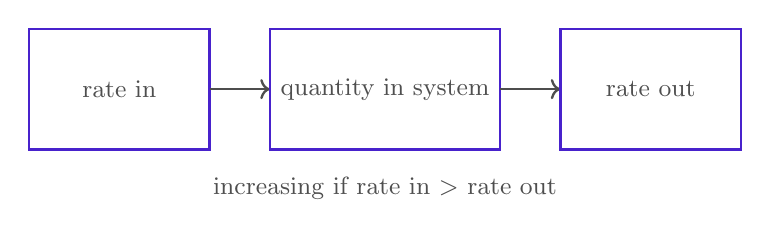
\begin{tikzpicture}[x=0.9cm,y=0.9cm]
    \draw[novelPurpleDark, line width=0.9pt] (0,0) rectangle (2.55,1.7);
    \node[text=npgray] at (1.275,0.85) {\small rate in};

    \draw[->, line width=0.85pt, npgray] (2.55,0.85)--(3.4,0.85);

    \draw[novelPurpleDark, line width=0.9pt] (3.4,0) rectangle (6.65,1.7);
    \node[text=npgray] at (5.025,0.85) {\small quantity in system};

    \draw[->, line width=0.85pt, npgray] (6.65,0.85)--(7.5,0.85);

    \draw[novelPurpleDark, line width=0.9pt] (7.5,0) rectangle (10.05,1.7);
    \node[text=npgray] at (8.775,0.85) {\small rate out};

    \node[text=npgray] at (5.025,-0.55) {\small increasing if rate in $>$ rate out};
\end{tikzpicture}
\end{center}
}

\newcommand{\relatedratesconefigure}{
\begin{center}
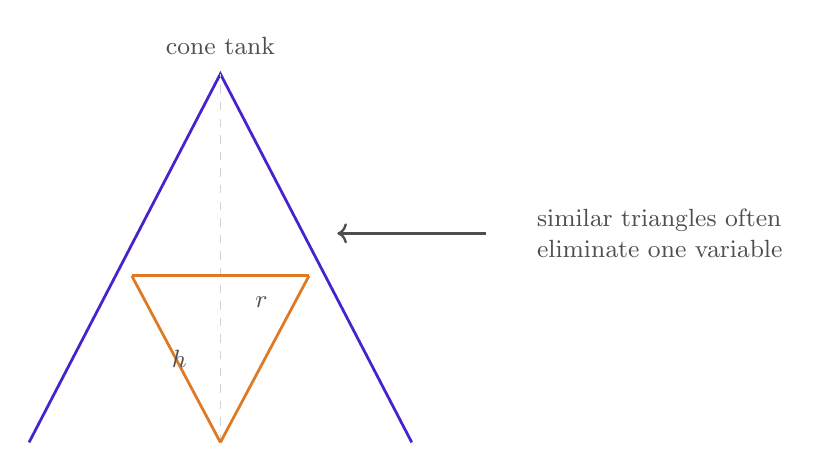
\begin{tikzpicture}[x=0.9cm,y=0.9cm]
    % outer cone
    \draw[novelPurpleDark, line width=1.0pt] (0,0)--(2.7,5.2)--(5.4,0);
    \draw[gray!35,dashed] (2.7,0)--(2.7,5.2);

    % water cone
    \draw[nporange, line width=1.0pt] (1.45,2.35)--(3.95,2.35);
    \draw[nporange, line width=1.0pt] (1.45,2.35)--(2.7,0);
    \draw[nporange, line width=1.0pt] (3.95,2.35)--(2.7,0);

    % labels
    \node[text=npgray] at (2.7,5.6) {\small cone tank};
    \node[text=npgray] at (3.28,1.98) {\small $r$};
    \node[text=npgray] at (2.12,1.18) {\small $h$};

    % side note with clean spacing
    \draw[->, line width=0.85pt, npgray] (6.45,2.95)--(4.35,2.95);
    \node[text=npgray, align=left] at (8.9,2.95) {\small similar triangles often\\[-0.1em]\small eliminate one variable};
\end{tikzpicture}
\end{center}
}

\newcommand{\linearapproxfigure}{
\begin{center}
\begin{tikzpicture}[x=0.9cm,y=0.9cm]
    % axes
    \draw[novelPurpleDark, line width=0.95pt, ->] (-0.2,0)--(6.3,0) node[right] {$x$};
    \draw[novelPurpleDark, line width=0.95pt, ->] (0,-0.2)--(0,4.4) node[above] {$y$};

    % curve: chosen to have a clean local tangent picture
    % f(x)=0.10(x-1.2)^3+0.18(x-1.2)^2+0.85
    \draw[novelPurple, line width=1.25pt, smooth, samples=240, domain=0.55:5.4]
        plot (\x,{0.10*(\x-1.2)^3 + 0.18*(\x-1.2)^2 + 0.85});

    % point of tangency at x = 2.8
    \pgfmathsetmacro{\xc}{2.8}
    \pgfmathsetmacro{\yc}{0.10*(\xc-1.2)^3 + 0.18*(\xc-1.2)^2 + 0.85}

    % derivative: f'(x)=0.30(x-1.2)^2+0.36(x-1.2)
    \pgfmathsetmacro{\m}{0.30*(\xc-1.2)^2 + 0.36*(\xc-1.2)}

    % tangent line computed from slope at the point
    \draw[nporange, line width=1.0pt]
        (1.55,{\m*(1.55-\xc)+\yc}) -- (4.95,{\m*(4.95-\xc)+\yc});

    % tangency point
    \fill[npred] (\xc,\yc) circle (1.55pt);

    % labels
    \node[text=npgray] at (4.55,2.65) {\small tangent line approximation};
    \node[text=npgray] at (3.55,1.35) {\small curve};
\end{tikzpicture}
\end{center}
}

\newcommand{\underoverfigure}{
\begin{center}
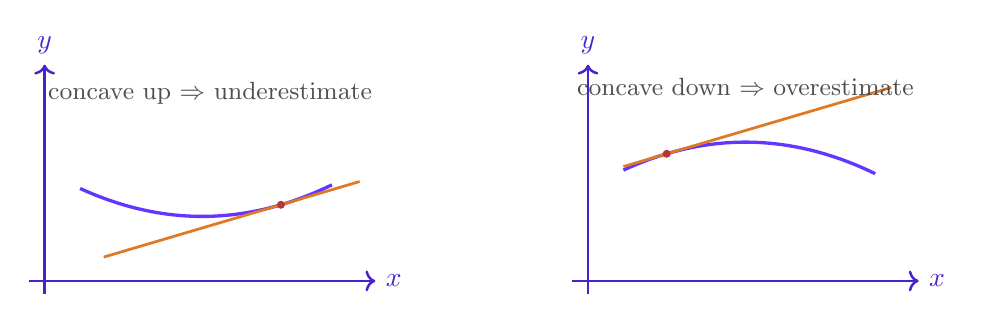
\begin{tikzpicture}[x=1cm,y=0.82cm]

    % =========================
    % Left panel: concave up => underestimate
    % =========================
    \begin{scope}[shift={(0,0)}]
        % axes
        \draw[novelPurpleDark, line width=0.9pt, ->] (-0.2,0)--(4.2,0) node[right] {$x$};
        \draw[novelPurpleDark, line width=0.9pt, ->] (0,-0.2)--(0,3.35) node[above] {$y$};

        % curve: y = 0.18(x-2)^2 + 1
        \draw[novelPurple, line width=1.2pt, smooth, samples=220, domain=0.45:3.65]
            plot (\x,{0.18*(\x-2)^2+1.0});

        % tangent point at x = 3
        \pgfmathsetmacro{\xa}{3.0}
        \pgfmathsetmacro{\ya}{0.18*(\xa-2)^2+1.0}
        % derivative = 0.36(x-2), so slope at x=3 is 0.36
        \draw[nporange, line width=1.0pt] (0.75,{0.36*(0.75-3)+\ya}) -- (4.0,{0.36*(4.0-3)+\ya});

        % tangency point
        \fill[npred] (\xa,\ya) circle (1.45pt);

        % label
        \node[text=npgray] at (2.1,2.9) {\small concave up $\Rightarrow$ underestimate};
    \end{scope}

    % =========================
    % Right panel: concave down => overestimate
    % =========================
    \begin{scope}[shift={(6.9,0)}]
        % axes
        \draw[novelPurpleDark, line width=0.9pt, ->] (-0.2,0)--(4.2,0) node[right] {$x$};
        \draw[novelPurpleDark, line width=0.9pt, ->] (0,-0.2)--(0,3.35) node[above] {$y$};

        % curve: y = -0.18(x-2)^2 + 2.15
        \draw[novelPurple, line width=1.2pt, smooth, samples=220, domain=0.45:3.65]
            plot (\x,{-0.18*(\x-2)^2+2.15});

        % tangent point at x = 1
        \pgfmathsetmacro{\xb}{1.0}
        \pgfmathsetmacro{\yb}{-0.18*(\xb-2)^2+2.15}
        % derivative = -0.36(x-2), so slope at x=1 is 0.36
        \draw[nporange, line width=1.0pt] (0.45,{0.36*(0.45-1)+\yb}) -- (3.85,{0.36*(3.85-1)+\yb});

        % tangency point
        \fill[npred] (\xb,\yb) circle (1.45pt);

        % label
        \node[text=npgray] at (2.0,3.0) {\small concave down $\Rightarrow$ overestimate};
    \end{scope}

\end{tikzpicture}
\end{center}
}

\newcommand{\lhospitalfigure}{
\begin{center}
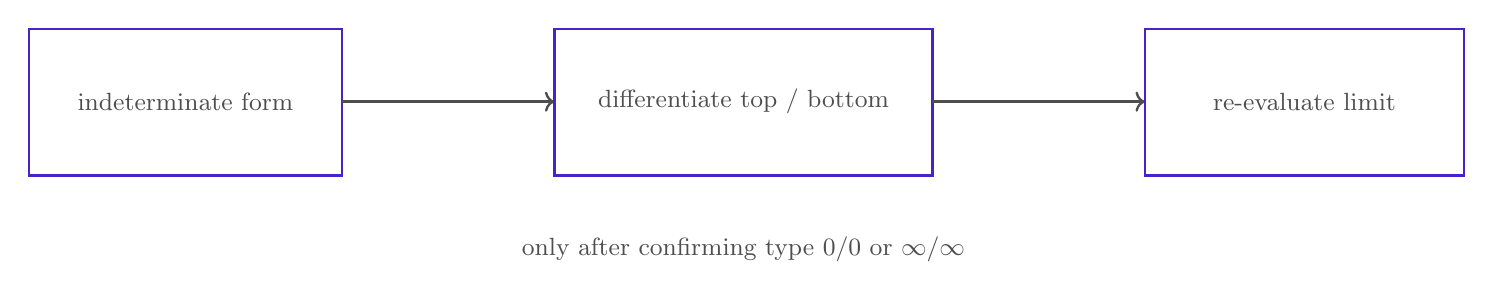
\begin{tikzpicture}[x=1.5cm,y=1.2cm]
    % first box
    \draw[novelPurpleDark, line width=0.9pt] (0,0) rectangle (2.65,1.55);
    \node[text=npgray] at (1.325,0.78) {\small indeterminate form};

    % arrow 1
    \draw[->, line width=0.85pt, npgray] (2.65,0.78)--(4.45,0.78);

    % second box
    \draw[novelPurpleDark, line width=0.9pt] (4.45,0) rectangle (7.65,1.55);
    \node[text=npgray] at (6.05,0.78) {\small differentiate top / bottom};

    % arrow 2
    \draw[->, line width=0.85pt, npgray] (7.65,0.78)--(9.45,0.78);

    % third box
    \draw[novelPurpleDark, line width=0.9pt] (9.45,0) rectangle (12.15,1.55);
    \node[text=npgray] at (10.8,0.78) {\small re-evaluate limit};

    % bottom note
    \node[text=npgray] at (6.05,-0.78) {\small only after confirming type $0/0$ or $\infty/\infty$};
\end{tikzpicture}
\end{center}
}

% =========================
% Document
% =========================
\begin{document}

\begin{titlepage}
\centering
\vspace*{2.0cm}

{\fontsize{28}{32}\selectfont\bfseries\color{novelPurpleDark} AP Calculus AB\par}
\vspace{0.35cm}
{\fontsize{28}{32}\selectfont\bfseries\color{novelPurpleDark} Unit 4: Application of Differentiation\par}


\begin{center}
    

\vspace{1.0cm}
\unitfourcoverfigure
\end{center}

\vfill

\begin{minipage}{0.84\textwidth}
\begin{notebox}{Design Goals for This Revision}
\begin{itemize}
    \item Preserve the original 4.1--4.6 flow from the first draft.
    \item Upgrade each section into a polished Novel Prep handout with clearer concept-building.
    \item Rebuild the weak TikZ figures so spacing, labels, and proportions look more like a textbook.
    \item Keep the chapter practical and AP-oriented, with strong contextual interpretation.
\end{itemize}
\end{notebox}
\end{minipage}

\vfill

{\large\textbf{Novel Prep Learning Center}}\\[0.25em]
{\large J. Z}

\end{titlepage}

\tableofcontents
\newpage

\setcounter{section}{3}
\section{Application of Differentiation}

\begin{theorybox}{Big Idea}
Unit 4 moves from computing derivatives to \emph{using} derivatives.
The derivative is no longer just an algebraic quantity; it becomes a language for motion, rate, approximation, and applied decision-making.
\end{theorybox}

\begin{notebox}{Teaching Philosophy for This Unit}
Students should learn to ask:
\begin{itemize}
    \item What does the derivative mean in this context?
    \item What are the units?
    \item What is changing, and what is causing that change?
    \item When can a tangent line replace the original curve?
\end{itemize}
\end{notebox}

% =========================================================
\unitchapter{Interpreting the Meaning of the Derivative}

\noindent\textbf{Why This Section Matters}

\smallskip

The first interpretation of the derivative is \emph{instantaneous rate of change}. If a quantity depends on another quantity, then the derivative tells how fast the output is changing at a particular input value.

\unitsubtopic{Units of the Derivative}

\begin{theorybox}{Theorem 4.1.1 --- Units of the Derivative}
If $y=f(x)$ and $y$ is measured in units $P$ while $x$ is measured in units $Q$, then
\[
\frac{dy}{dx}
\]
has units
\[
\frac{\text{units of }y}{\text{units of }x}=\frac{P}{Q}.
\]
For example, if $y$ is measured in feet and $x$ in seconds, then $y'=f'(x)$ has units feet per second.
\end{theorybox}

\unitsfigure

\begin{summarybox}{Core Interpretation}
\[
f'(a)=\text{instantaneous rate of change of }f\text{ at }x=a
\]
Read it as: “At this instant, the output is changing at this many output-units per input-unit.”
\end{summarybox}

\example{Manufacturing interpretation}
What do $P(1000)=500$ and $P'(1000)=0.25$ mean? Approximate $P(1100)$.

\solution
The equation $P(1000)=500$ means selling 1000 widgets returns a profit of $\$500. The value $P'(1000)=0.25$ means that near 1000 widgets, profit is increasing at a rate of $\$0.25 per widget.

Using a linear estimate,
\[
P(1100)\approx P(1000)+P'(1000)(1100-1000)=500+0.25(100)=525.
\]
So the estimated profit is
\[
\boxed{\$525.}
\]

\begin{notebox}{Teacher Emphasis}
The derivative is not the value of the function. It is the \emph{rate at which the function value is changing}.
\end{notebox}

% =========================================================
\unitchapter{Straight Line Motion (Position, Velocity, and Acceleration)}

\begin{theorybox}{Theorem 4.2.1 --- Straight Line Motion}
If $s=f(t)$ is the position of a particle moving in a straight line, then:
\begin{enumerate}
    \item Average velocity over a time interval is
    \[
    \frac{\Delta s}{\Delta t}.
    \]
    \item Instantaneous velocity is
    \[
    v(t)=\frac{ds}{dt}=s'(t).
    \]
    \item Instantaneous acceleration is
    \[
    a(t)=v'(t)=s''(t).
    \]
\end{enumerate}
\end{theorybox}

\motionoverviewfigure

\begin{notebox}{Vector Language Simplified for AP Calculus}
Velocity carries both magnitude and direction.
In one-dimensional motion:
\begin{itemize}
    \item $v(t)>0$ means moving to the right / forward.
    \item $v(t)<0$ means moving to the left / backward.
    \item $v(t)=0$ means the particle is at rest.
\end{itemize}
\end{notebox}

\begin{summarybox}{Speeding Up vs. Slowing Down}
\begin{itemize}
    \item The particle is \textbf{speeding up} when velocity and acceleration have the same sign.
    \item The particle is \textbf{slowing down} when velocity and acceleration have opposite signs.
\end{itemize}
\end{summarybox}

\speedingfigure

\example{Position of a particle}
A particle moves along the $x$-axis with position
\[
x(t)=\frac13 t^3-\frac52 t^2+4t+6,\qquad 0\le t\le 5.
\]
(a) When is the particle at rest?  
(b) When is the particle moving left?  
(c) At $t=3$, is it speeding up or slowing down?

\solution
Velocity:
\[
v(t)=x'(t)=t^2-5t+4=(t-1)(t-4).
\]

(a) At rest when $v(t)=0$:
\[
t=1,\quad t=4.
\]

(b) Moving left when $v(t)<0$:
\[
1<t<4.
\]

(c) Acceleration:
\[
a(t)=v'(t)=2t-5.
\]
At $t=3$,
\[
v(3)=(3-1)(3-4)=-2,
\qquad
 a(3)=1.
\]
Since velocity is negative and acceleration is positive, the particle is
\[
\boxed{\text{slowing down}.}
\]

\example{Another motion checklist problem}
The position of a particle is
\[
s(t)=t^3-6t^2+9t.
\]
Find the velocity, the times when the particle is at rest, and the intervals when it moves forward.

\solution
\[
v(t)=s'(t)=3t^2-12t+9=3(t-1)(t-3).
\]
At rest when
\[
t=1,\quad t=3.
\]
Moving forward when $v(t)>0$:
\[
(-\infty,1)\cup(3,\infty).
\]

% =========================================================
\unitchapter{Rates of Change in Applied Contexts Other Than Motion}

\begin{theorybox}{Definition 4.3.1 --- Rate of Change}
The rate-of-change function is the derivative of the original function. It may be given by an equation, a table, or a graph.
\end{theorybox}

\noindent
Outside motion, derivatives describe changing populations, changing volume, changing profit, changing temperature, and many other contextual quantities.

\rateinoutfigure

\begin{notebox}{Rate In and Rate Out}
Some quantities are controlled by two competing rates.
\begin{itemize}
    \item If rate in $>$ rate out, the quantity increases.
    \item If rate in $<$ rate out, the quantity decreases.
    \item If rate in $=$ rate out, the quantity is momentarily not changing.
\end{itemize}
\end{notebox}

\example{Amusement park rate}
People enter an amusement park at rate
\[
E(t)=\frac{15600}{t^2-24t+160},
\]
where $E$ is in people per hour and $t$ is in hours after midnight. Find $E'(11)$ and interpret it.

\solution
Differentiate:
\[
E'(t)=\frac{-15600(2t-24)}{(t^2-24t+160)^2}.
\]
Then
\[
E'(11)=\frac{31200}{289}\approx 107.96.
\]
Interpretation: at 11 AM, the rate at which people are entering the park is increasing by about
\[
\boxed{108\text{ people/hour}^2.}
\]

\example{Penguin population}
A penguin population has birth rate
\[
B(t)=1000e^{0.06t}
\]
and death rate
\[
D(t)=250e^{0.1t}.
\]
Determine whether the population is increasing or decreasing at $t=5$.

\solution
Evaluate:
\[
B(5)=1000e^{0.3}\approx 1349.86,
\qquad
D(5)=250e^{0.5}\approx 412.18.
\]
Because $B(5)>D(5)$, the population is
\[
\boxed{\text{increasing at } t=5.}
\]

% =========================================================
\unitchapter{Related Rates}

\unitsubtopic{Introduction to Related Rates}

\begin{theorybox}{Core Idea of Related Rates}
When two or more variables are connected by one equation and all of them change with time, their rates are related through implicit differentiation and the Chain Rule.
\end{theorybox}

\begin{notebox}{Template Language}
In related rates, almost every variable should be thought of as a function of time:
\[
x=x(t),\qquad y=y(t),\qquad r=r(t),\qquad h=h(t),\dots
\]
That is why differentiating with respect to $t$ introduces terms like
\[
\frac{dx}{dt},\quad \frac{dy}{dt},\quad \frac{dr}{dt},\quad \frac{dh}{dt}.
\]
\end{notebox}

\example{Two rates that are related}
The variables $x$ and $y$ satisfy
\[
y=x^2+3.
\]
Find $\dfrac{dy}{dt}$ when $x=1$ and $\dfrac{dx}{dt}=2$.

\solution
Differentiate both sides with respect to $t$:
\[
\frac{dy}{dt}=2x\frac{dx}{dt}.
\]
Substitute $x=1$ and $\dfrac{dx}{dt}=2$:
\[
\frac{dy}{dt}=2(1)(2)=\boxed{4}.
\]

\unitsubtopic{Problem Solving with Related Rates}

\begin{skillbox}{Guidelines for Solving Related-Rate Problems}
\begin{enumerate}
    \item Identify all given quantities and the quantity to be found.
    \item Draw a diagram and label variables carefully.
    \item Write an equation relating the variables.
    \item Differentiate implicitly with respect to time.
    \item Substitute known values only \emph{after} differentiating.
    \item Solve for the required rate and include units.
\end{enumerate}
\end{skillbox}

\relatedratesconefigure

\begin{summarybox}{Common Translation Patterns}
\renewcommand{\arraystretch}{1.38}
\begin{tabularx}{\textwidth}{@{}p{0.44\textwidth}X@{}}
\toprule
\textbf{Verbal statement} & \textbf{Mathematical model}\\
\midrule
Car travels 50 miles per hour & $\dfrac{dx}{dt}=50$ mi/h\\
Water enters a tank at 10 m$^3$/h & $\dfrac{dV}{dt}=10$ m$^3$/h\\
Angle changes at 25 rev/min & $\dfrac{d\theta}{dt}=25(2\pi)$ rad/min\\
Population increases by 2000 per hour & $\dfrac{dx}{dt}=2000$ units/h\\
\bottomrule
\end{tabularx}
\end{summarybox}

\example{Airplane tracked by radar}
An airplane flies directly over a radar station. The slant distance $s$ is decreasing at 400 mi/h when $s=10$ miles and the altitude is 6 miles. Find the airplane's speed.

\solution
Let $x$ be the horizontal distance from the station. Then
\[
x^2+6^2=s^2.
\]
When $s=10$,
\[
x=\sqrt{10^2-6^2}=8.
\]
Differentiate:
\[
2x\frac{dx}{dt}=2s\frac{ds}{dt}.
\]
So
\[
\frac{dx}{dt}=\frac{s}{x}\frac{ds}{dt}.
\]
Substitute:
\[
\frac{dx}{dt}=\frac{10}{8}(-400)=-500.
\]
The speed is
\[
\boxed{500\text{ mi/h}.}
\]

\example{Ripples in a pond}
A ripple radius increases at 1 ft/s. When the radius is 4 ft, how fast is the disturbed area changing?

\solution
\[
A=\pi r^2
\]
Differentiate with respect to time:
\[
\frac{dA}{dt}=2\pi r\frac{dr}{dt}.
\]
Substitute $r=4$ and $\dfrac{dr}{dt}=1$:
\[
\frac{dA}{dt}=2\pi(4)(1)=\boxed{8\pi\text{ ft}^2/\text{s}}.
\]

\example{Rising water level in a cone}
An inverted cone has base radius 2 m and height 4 m. Water is pumped in at 2 m$^3$/min. Find $\dfrac{dh}{dt}$ when $h=3$.

\solution
Volume of cone:
\[
V=\frac13\pi r^2h.
\]
Use similar triangles:
\[
\frac{r}{h}=\frac24=\frac12
\Rightarrow r=\frac h2.
\]
Then
\[
V=\frac13\pi\left(\frac h2\right)^2h=\frac{\pi}{12}h^3.
\]
Differentiate:
\[
\frac{dV}{dt}=\frac\pi4 h^2\frac{dh}{dt}.
\]
Substitute $\dfrac{dV}{dt}=2$ and $h=3$:
\[
2=\frac\pi4(9)\frac{dh}{dt}.
\]
So
\[
\frac{dh}{dt}=\frac{8}{9\pi}\approx 0.28\text{ m/min}.
\]

% =========================================================
\unitchapter{Linear Approximation and Differentials}

\unitsubtopic{Tangent Line Approximations}

\begin{theorybox}{Tangent Line Approximation}
If $f$ is differentiable at $x=c$, then the tangent line at $(c,f(c))$ is
\[
y-f(c)=f'(c)(x-c),
\]
or equivalently
\[
L(x)=f(c)+f'(c)(x-c).
\]
Near $x=c$, the function value is approximated by
\[
f(x)\approx L(x).
\]
\end{theorybox}

\linearapproxfigure

\example{Using a tangent line approximation}
Find the tangent line approximation of $f(x)=1+\sin x$ at $(0,1)$.

\solution
\[
f'(x)=\cos x.
\]
At $x=0$,
\[
f(0)=1,\qquad f'(0)=1.
\]
So the tangent line is
\[
L(x)=1+1(x-0)=\boxed{1+x}.
\]

\example{Estimate a nearby value}
For a differentiable function $g$, suppose $g(2)=7$ and $g'(2)=-3$. Estimate $g(2.1)$.

\solution
\[
L(x)=g(2)+g'(2)(x-2)=7-3(x-2).
\]
Thus
\[
g(2.1)\approx L(2.1)=7-3(0.1)=\boxed{6.7}.
\]

\unitsubtopic{Underestimate or Overestimate}

\begin{summarybox}{Concavity Controls the Error Direction}
\begin{itemize}
    \item If $f''(x)>0$ near the point, then the tangent line approximation is typically an \textbf{underestimate}.
    \item If $f''(x)<0$ near the point, then the tangent line approximation is typically an \textbf{overestimate}.
\end{itemize}
\end{summarybox}

\underoverfigure

\begin{notebox}{Common Mistake}
To decide whether a tangent line approximation is an overestimate or underestimate, look at the \textbf{second derivative}, not the first derivative.
\end{notebox}

\example{Approximation direction}
Suppose $g(2)=7$, $g'(2)=-3$, and $g''(2)=-5$.
(a) Estimate $g(2.1)$.  
(b) Is the estimate an overestimate or underestimate?

\solution
(a)
\[
L(x)=7-3(x-2),
\]
so
\[
L(2.1)=6.7.
\]

(b) Since $g''(2)=-5<0$, the graph is concave down, so the tangent line lies above the curve near $x=2$.
Thus the estimate is an
\[
\boxed{\text{overestimate}.}
\]

\unitsubtopic{Differentials}

\begin{theorybox}{Differentials}
If $y=f(x)$ is differentiable, then the differential of $x$ is $dx$, and the differential of $y$ is
\[
dy=f'(x)\,dx.
\]
When $dx$ is small,
\[
\Delta y\approx dy.
\]
\end{theorybox}

\begin{notebox}{Visual Meaning of a Differential}
The exact change is
\[
\Delta y=f(x+\Delta x)-f(x),
\]
but the tangent-line-based approximation is
\[
dy=f'(x)dx.
\]
So a differential is the tangent-line prediction for a small nearby change.
\end{notebox}

\begin{summarybox}{Interpretation of Differentials}
\[
dy=f'(x)dx
\]
means “approximate change in the output” equals “instantaneous rate of change” times “small change in the input.”
\end{summarybox}

% =========================================================
\unitchapter{L'Hospital's Rule}

\begin{theorybox}{Theorem 4.6.1 --- L'Hospital's Rule}
Suppose $f$ and $g$ are differentiable near $a$, and suppose the quotient
\[
\frac{f(x)}{g(x)}
\]
produces one of the indeterminate forms
\[
\frac00 \qquad \text{or} \qquad \frac{\infty}{\infty}.
\]
Then, if the resulting limit exists,
\[
\lim_{x\to a}\frac{f(x)}{g(x)}=\lim_{x\to a}\frac{f'(x)}{g'(x)}.
\]
\end{theorybox}

\lhospitalfigure

\begin{notebox}{When You May Use It}
Use L'Hospital's Rule only after:
\begin{itemize}
    \item substituting into the original quotient,
    \item confirming the form is $0/0$ or $\infty/\infty$,
    \item and verifying both numerator and denominator are differentiable near the point.
\end{itemize}
\end{notebox}

\example{A logarithmic limit}
Find
\[
\lim_{x\to 1}\frac{\ln x}{x-1}.
\]

\solution
Substitute $x=1$:
\[
\ln 1=0,\qquad 1-1=0.
\]
So the limit is $0/0$.
Apply L'Hospital's Rule:
\[
\lim_{x\to1}\frac{\ln x}{x-1}=\lim_{x\to1}\frac{1/x}{1}=\lim_{x\to1}\frac1x=\boxed{1}.
\]

\example{An exponential-over-polynomial limit}
Find
\[
\lim_{x\to\infty}\frac{e^x}{x^2}.
\]

\solution
As $x\to\infty$ we have $\infty/\infty$.
Apply L'Hospital once:
\[
\lim_{x\to\infty}\frac{e^x}{x^2}=\lim_{x\to\infty}\frac{e^x}{2x}.
\]
Still $\infty/\infty$, so apply again:
\[
\lim_{x\to\infty}\frac{e^x}{2x}=\lim_{x\to\infty}\frac{e^x}{2}=\boxed{\infty}.
\]

\example{Table / chain-rule style L'Hospital problem}
Suppose selected values of a differentiable function satisfy $f(5)=0$ and $f'(5)=7$. Find
\[
\lim_{x\to3}\frac{f(2x-1)}{x^2-9}.
\]

\solution
Substitute $x=3$:
\[
f(2\cdot 3-1)=f(5)=0,
\qquad
3^2-9=0.
\]
So the form is $0/0$.
Apply L'Hospital's Rule:
\[
\lim_{x\to3}\frac{f(2x-1)}{x^2-9}
=
\lim_{x\to3}\frac{f'(2x-1)\cdot 2}{2x}.
\]
Now substitute $x=3$:
\[
\frac{f'(5)\cdot 2}{6}=\frac{7\cdot 2}{6}=\boxed{\frac73}.
\]

% =========================================================
\newpage
\subsection{Unit 4 Summary / Formula Sheet}

\begin{summarybox}{Unit 4 Master Summary Sheet}
\renewcommand{\arraystretch}{1.35}
\begin{tabularx}{\textwidth}{@{}p{0.37\textwidth}X@{}}
\toprule
\textbf{Topic} & \textbf{Key Formula / Idea} \\
\midrule
Meaning of derivative & instantaneous rate of change \\
Derivative units & output units / input units \\
Position, velocity, acceleration & $v=s'$, $a=v'=s''$ \\
Speeding up/down & same sign of $v$ and $a$ means speeding up \\
Rate in / rate out & compare competing rates \\
Related rates & differentiate linked variables with respect to time \\
Linear approximation & $L(x)=f(c)+f'(c)(x-c)$ \\
Differentials & $dy=f'(x)dx$ \\
Over/under estimate & use the sign of $f''$ \\
L'Hospital's Rule & only for $0/0$ or $\infty/\infty$ \\
\bottomrule
\end{tabularx}
\end{summarybox}

\vspace{1em}

\begin{summarybox}{Big Strategy Ladder}
\begin{itemize}
    \item First interpret what the derivative means in context.
    \item Then attach correct units.
    \item In related rates, write a relationship before differentiating.
    \item In linear approximation, use the tangent line only near the base point.
    \item In L'Hospital, always identify the indeterminate form first.
\end{itemize}
\end{summarybox}

% =========================================================
\unitchapter{Homework / Class Exercises}

\section*{Homework A --- Interpreting Rates and Motion}

\begin{enumerate}
    \item A company's profit \(P(x)\), in dollars, depends on the number of products sold \(x\).  
    Suppose \(P(500)=1200\) and \(P'(500)=3.5\).
    \begin{enumerate}
        \item Interpret \(P(500)\).
        \item Interpret \(P'(500)\), including units.
        \item Use a linear approximation to estimate \(P(520)\).
    \end{enumerate}

    \item The position of a particle moving on the \(x\)-axis is
    \[
    s(t)=t^3-6t^2+9t+1,\qquad 0\le t\le 5.
    \]
    \begin{enumerate}
        \item Find the velocity function.
        \item Find the acceleration function.
        \item Determine when the particle is at rest.
        \item Determine the intervals when the particle moves to the right.
        \item Determine whether the particle is speeding up or slowing down at \(t=4\).
    \end{enumerate}

    \item A car moves along a straight road with velocity
    \[
    v(t)=t^2-4t+3,\qquad 0\le t\le 6.
    \]
    \begin{enumerate}
        \item Find all times when the car changes direction.
        \item Find the acceleration at those times.
        \item Determine the intervals when the car is speeding up.
    \end{enumerate}

    \item A quantity \(Q(t)\) is measured in liters and time \(t\) is measured in minutes.
    Explain the meaning and units of each of the following:
    \[
    Q(10)=48,\qquad Q'(10)=-1.6.
    \]
\end{enumerate}

\bigskip
\newpage
\section*{Homework B --- Rates of Change in Context and Related Rates}

\begin{enumerate}
    \setcounter{enumi}{4}

    \item The number of people in a stadium is changing according to
    \[
    N'(t)=500e^{-0.2t}-120,
    \]
    where \(t\) is measured in hours.
    \begin{enumerate}
        \item At what rate is the number of people changing at \(t=2\)?
        \item Is the number of people increasing or decreasing at \(t=2\)?
    \end{enumerate}

    \item Water leaks from a tank at 4 m\(^3\)/min while water is pumped in at a rate
    \[
    R(t)=10-0.5t
    \]
    m\(^3\)/min.
    \begin{enumerate}
        \item Write an expression for the net rate of change of the water volume.
        \item At what rate is the volume changing when \(t=6\)?
        \item Is the volume increasing or decreasing at that time?
    \end{enumerate}

    \item A ladder 13 ft long leans against a wall. The bottom of the ladder slides away from the wall at 2 ft/s.
    How fast is the top of the ladder sliding down the wall when the bottom is 5 ft from the wall?

    \item The radius of a spherical balloon increases at 0.2 cm/s.  
    How fast is the volume changing when the radius is 10 cm?

    \item A spotlight is on the ground 20 m from a wall. A person 2 m tall walks from the spotlight toward the wall at 1.5 m/s.
    How fast is the height of the shadow on the wall changing when the person is 8 m from the light?

    \item An inverted cone has height 12 m and radius 6 m. Water is poured in at a rate of 3 m\(^3\)/min.
    How fast is the water level rising when the water depth is 4 m?
\end{enumerate}

\bigskip
\newpage
\section*{Homework C --- Linear Approximation, Differentials, and L'Hospital's Rule}

\begin{enumerate}
    \setcounter{enumi}{10}

    \item Find the linearization of
    \[
    f(x)=\sqrt{x+5}
    \]
    at \(x=4\). Then use it to approximate \(\sqrt{9.3}\).

    \item For
    \[
    f(x)=\ln x,
    \]
    find the tangent line approximation at \(x=1\), and use it to estimate \(\ln(1.08)\).

    \item Suppose \(g(3)=10\), \(g'(3)=-4\), and \(g''(3)=6\).
    \begin{enumerate}
        \item Estimate \(g(3.1)\) using linear approximation.
        \item Determine whether the estimate is an overestimate or an underestimate.
    \end{enumerate}

    \item Use differentials to approximate the change in area of a circle when the radius changes from 5 cm to 5.1 cm.

    \item Use L'Hospital's Rule to evaluate
    \[
    \lim_{x\to 0}\frac{e^x-1-x}{x^2}.
    \]

    \item Use L'Hospital's Rule to evaluate
    \[
    \lim_{x\to \infty}\frac{\ln x}{x^{1/3}}.
    \]

    \item Suppose \(f(2)=0\) and \(f'(2)=5\). Evaluate
    \[
    \lim_{x\to 1}\frac{f(2x)}{x-1}.
    \]

    \item Use a tangent line approximation to estimate \((1.98)^4\).
\end{enumerate}

\bigskip
\newpage
\section*{Challenge Problems}

\begin{enumerate}
    \setcounter{enumi}{18}

    \item A particle has position
    \[
    s(t)=t^4-8t^3+18t^2.
    \]
    Find all times when the particle is at rest, and determine whether it is moving left or right immediately after each of those times.

    \item A right circular cylinder is expanding so that its radius increases at 0.4 cm/s and its height decreases at 0.1 cm/s.
    If the radius is 5 cm and the height is 12 cm, find the rate of change of the volume.

    \item Explain why linear approximation works best only near the point of tangency.

    \item Find
    \[
    \lim_{x\to 0}\frac{\sin x - x}{x^3}.
    \]
\end{enumerate}

% =========================================================

\unitchapter{Homework Answer Key}

\section*{Homework A --- Interpreting Rates and Motion}

\begin{enumerate}
    \item 
    \begin{enumerate}
        \item \(P(500)=1200\) means selling 500 products gives a profit of \$1200.
        \item \(P'(500)=3.5\) means that near 500 products, profit is increasing at about \$3.50 per product.
        \item Linear approximation:
        \[
        P(520)\approx P(500)+P'(500)(520-500)=1200+3.5(20)=1270.
        \]
        So the estimate is
        \[
        \boxed{1270}.
        \]
    \end{enumerate}

    \item 
    \[
    s(t)=t^3-6t^2+9t+1
    \]
    \[
    v(t)=s'(t)=3t^2-12t+9=3(t-1)(t-3)
    \]
    \[
    a(t)=v'(t)=6t-12
    \]
    At rest when
    \[
    v(t)=0 \Rightarrow t=1,\ 3.
    \]
    Moving right when \(v(t)>0\):
    \[
    (0,1)\cup(3,5].
    \]
    At \(t=4\),
    \[
    v(4)=3(16)-48+9=9>0,\qquad a(4)=24-12=12>0.
    \]
    Since velocity and acceleration have the same sign, the particle is
    \[
    \boxed{\text{speeding up at } t=4.}
    \]

    \item 
    \[
    v(t)=t^2-4t+3=(t-1)(t-3)
    \]
    Direction changes when velocity changes sign, so at
    \[
    t=1,\ 3.
    \]
    Acceleration:
    \[
    a(t)=v'(t)=2t-4.
    \]
    Thus
    \[
    a(1)=-2,\qquad a(3)=2.
    \]
    Sign chart for \(v\) and \(a\):
    \begin{itemize}
        \item On \((0,1)\): \(v>0,\ a<0\) \(\Rightarrow\) slowing down
        \item On \((1,2)\): \(v<0,\ a<0\) \(\Rightarrow\) speeding up
        \item On \((2,3)\): \(v<0,\ a>0\) \(\Rightarrow\) slowing down
        \item On \((3,6)\): \(v>0,\ a>0\) \(\Rightarrow\) speeding up
    \end{itemize}
    So the car is speeding up on
    \[
    \boxed{(1,2)\cup(3,6).}
    \]

    \item 
    \(Q(10)=48\) means that at \(t=10\) minutes, the quantity is 48 liters.  
    \(Q'(10)=-1.6\) means that at \(t=10\), the quantity is decreasing at
    \[
    \boxed{1.6\text{ liters per minute}.}
    \]
\end{enumerate}

\bigskip

\section*{Homework B --- Rates of Change in Context and Related Rates}

\begin{enumerate}
    \setcounter{enumi}{4}

    \item 
    \[
    N'(t)=500e^{-0.2t}-120
    \]
    At \(t=2\),
    \[
    N'(2)=500e^{-0.4}-120\approx 500(0.6703)-120\approx 215.15.
    \]
    So the number of people is changing at about
    \[
    \boxed{215.15\text{ people per hour}}
    \]
    and since this is positive, the number is
    \[
    \boxed{\text{increasing}.}
    \]

    \item 
    Net rate:
    \[
    \frac{dV}{dt}=R(t)-4=(10-0.5t)-4=6-0.5t.
    \]
    At \(t=6\),
    \[
    \frac{dV}{dt}=6-0.5(6)=3.
    \]
    So the volume is changing at
    \[
    \boxed{3\text{ m}^3/\text{min}}
    \]
    and is
    \[
    \boxed{\text{increasing}.}
    \]

    \item 
    Let \(x\) be the bottom distance and \(y\) the height of the top. Then
    \[
    x^2+y^2=13^2=169.
    \]
    Differentiate:
    \[
    2x\frac{dx}{dt}+2y\frac{dy}{dt}=0.
    \]
    So
    \[
    \frac{dy}{dt}=-\frac{x}{y}\frac{dx}{dt}.
    \]
    When \(x=5\),
    \[
    y=\sqrt{169-25}=12.
    \]
    Hence
    \[
    \frac{dy}{dt}=-\frac{5}{12}(2)=-\frac{5}{6}.
    \]
    So the top slides down at
    \[
    \boxed{\frac56\text{ ft/s downward}.}
    \]

    \item 
    Volume of a sphere:
    \[
    V=\frac43\pi r^3.
    \]
    Differentiate:
    \[
    \frac{dV}{dt}=4\pi r^2\frac{dr}{dt}.
    \]
    Substitute \(r=10\), \(\frac{dr}{dt}=0.2\):
    \[
    \frac{dV}{dt}=4\pi(100)(0.2)=80\pi.
    \]
    Therefore,
    \[
    \boxed{\frac{dV}{dt}=80\pi\text{ cm}^3/\text{s}.}
    \]

    \item 
    Let \(x\) be the distance from the light to the person, and \(y\) the height of the shadow on the wall.  
    By similar triangles,
    \[
    \frac{y}{20}=\frac{2}{20-x}.
    \]
    So
    \[
    y=\frac{40}{20-x}.
    \]
    Differentiate:
    \[
    \frac{dy}{dt}=40(20-x)^{-2}\frac{dx}{dt}.
    \]
    Since the person walks toward the wall,
    \[
    \frac{dx}{dt}=1.5.
    \]
    At \(x=8\),
    \[
    \frac{dy}{dt}=40(12)^{-2}(1.5)=\frac{60}{144}=\frac{5}{12}.
    \]
    So
    \[
    \boxed{\frac{dy}{dt}=\frac{5}{12}\text{ m/s}.}
    \]

    \item 
    For the cone,
    \[
    V=\frac13\pi r^2h.
    \]
    Since \(\frac{r}{h}=\frac{6}{12}=\frac12\), we have
    \[
    r=\frac h2.
    \]
    Then
    \[
    V=\frac13\pi\left(\frac h2\right)^2h=\frac{\pi}{12}h^3.
    \]
    Differentiate:
    \[
    \frac{dV}{dt}=\frac{\pi}{4}h^2\frac{dh}{dt}.
    \]
    Substitute \(\frac{dV}{dt}=3\), \(h=4\):
    \[
    3=\frac{\pi}{4}(16)\frac{dh}{dt}=4\pi\frac{dh}{dt}.
    \]
    So
    \[
    \frac{dh}{dt}=\frac{3}{4\pi}.
    \]
    Therefore,
    \[
    \boxed{\frac{dh}{dt}=\frac{3}{4\pi}\text{ m/min}.}
    \]
\end{enumerate}

\bigskip

\section*{Homework C --- Linear Approximation, Differentials, and L'Hospital's Rule}

\begin{enumerate}
    \setcounter{enumi}{10}

    \item 
    \[
    f(x)=\sqrt{x+5},\qquad f'(x)=\frac{1}{2\sqrt{x+5}}
    \]
    At \(x=4\),
    \[
    f(4)=3,\qquad f'(4)=\frac16.
    \]
    Linearization:
    \[
    L(x)=3+\frac16(x-4).
    \]
    Then
    \[
    \sqrt{9.3}=f(4.3)\approx L(4.3)=3+\frac16(0.3)=3.05.
    \]
    So
    \[
    \boxed{\sqrt{9.3}\approx 3.05.}
    \]

    \item 
    \[
    f(x)=\ln x,\qquad f'(x)=\frac1x
    \]
    At \(x=1\),
    \[
    f(1)=0,\qquad f'(1)=1.
    \]
    Tangent line approximation:
    \[
    L(x)=x-1.
    \]
    Then
    \[
    \ln(1.08)\approx 1.08-1=0.08.
    \]
    Thus
    \[
    \boxed{\ln(1.08)\approx 0.08.}
    \]

    \item 
    \begin{enumerate}
        \item
        \[
        L(x)=g(3)+g'(3)(x-3)=10-4(x-3).
        \]
        So
        \[
        g(3.1)\approx 10-4(0.1)=9.6.
        \]
        \item Since
        \[
        g''(3)=6>0,
        \]
        the graph is concave up, so the tangent line lies below the curve near \(x=3\). Therefore the estimate is an
        \[
        \boxed{\text{underestimate}.}
        \]
    \end{enumerate}

    \item 
    Area of a circle:
    \[
    A=\pi r^2.
    \]
    Differential:
    \[
    dA=2\pi r\,dr.
    \]
    Here
    \[
    r=5,\qquad dr=0.1.
    \]
    So
    \[
    dA=2\pi(5)(0.1)=\pi.
    \]
    Approximate change in area:
    \[
    \boxed{\pi\text{ cm}^2.}
    \]

    \item 
    \[
    \lim_{x\to 0}\frac{e^x-1-x}{x^2}
    \]
    Substitute \(x=0\):
    \[
    \frac{0}{0}.
    \]
    Apply L'Hospital:
    \[
    \lim_{x\to 0}\frac{e^x-1}{2x}
    \]
    Still \(\frac00\), so apply again:
    \[
    \lim_{x\to 0}\frac{e^x}{2}=\frac12.
    \]
    Therefore,
    \[
    \boxed{\frac12}.
    \]

    \item 
    \[
    \lim_{x\to\infty}\frac{\ln x}{x^{1/3}}
    \]
    This is \(\frac{\infty}{\infty}\). Apply L'Hospital:
    \[
    \lim_{x\to\infty}\frac{1/x}{\frac13 x^{-2/3}}
    =
    \lim_{x\to\infty}\frac{3x^{-1}}{x^{-2/3}}
    =
    \lim_{x\to\infty}\frac{3}{x^{1/3}}=0.
    \]
    So
    \[
    \boxed{0}.
    \]

    \item 
    We evaluate
    \[
    \lim_{x\to 1}\frac{f(2x)}{x-1}.
    \]
    Since \(f(2)=0\), substitution gives \(\frac00\). Apply L'Hospital:
    \[
    \lim_{x\to1}\frac{2f'(2x)}{1}=2f'(2)=2(5)=10.
    \]
    Thus
    \[
    \boxed{10}.
    \]

    \item 
    Let
    \[
    f(x)=x^4.
    \]
    Then
    \[
    f'(x)=4x^3.
    \]
    At \(x=2\),
    \[
    f(2)=16,\qquad f'(2)=32.
    \]
    Linearization:
    \[
    L(x)=16+32(x-2).
    \]
    Estimate:
    \[
    (1.98)^4=f(1.98)\approx 16+32(-0.02)=16-0.64=15.36.
    \]
    So
    \[
    \boxed{(1.98)^4\approx 15.36.}
    \]
\end{enumerate}

\bigskip

\section*{Challenge Problems}

\begin{enumerate}
    \setcounter{enumi}{18}

    \item 
    \[
    s(t)=t^4-8t^3+18t^2
    \]
    Velocity:
    \[
    v(t)=s'(t)=4t^3-24t^2+36t=4t(t-3)^2.
    \]
    At rest when
    \[
    t=0,\ 3.
    \]
    Since \((t-3)^2\ge 0\), the sign of \(v\) depends on \(t\).
    \begin{itemize}
        \item Immediately after \(t=0\), \(v>0\), so the particle moves right.
        \item At \(t=3\), the sign does not change, so it is still moving right immediately after.
    \end{itemize}

    \item 
    Cylinder volume:
    \[
    V=\pi r^2h.
    \]
    Differentiate:
    \[
    \frac{dV}{dt}=2\pi rh\frac{dr}{dt}+\pi r^2\frac{dh}{dt}.
    \]
    Substitute \(r=5\), \(h=12\), \(\frac{dr}{dt}=0.4\), \(\frac{dh}{dt}=-0.1\):
    \[
    \frac{dV}{dt}=2\pi(5)(12)(0.4)+\pi(25)(-0.1).
    \]
    \[
    \frac{dV}{dt}=48\pi-2.5\pi=45.5\pi.
    \]
    So
    \[
    \boxed{\frac{dV}{dt}=45.5\pi\text{ cm}^3/\text{s}.}
    \]

    \item 
    Linear approximation is based on the tangent line at one point. The tangent line matches the function best very close to that point, but as you move farther away, the curve bends away from the line. Therefore, the approximation becomes less accurate farther from the point of tangency.

    \item 
    \[
    \lim_{x\to 0}\frac{\sin x-x}{x^3}
    \]
    Substitute \(x=0\): \(\frac00\). Apply L'Hospital:
    \[
    \lim_{x\to0}\frac{\cos x-1}{3x^2}
    \]
    Still \(\frac00\). Apply again:
    \[
    \lim_{x\to0}\frac{-\sin x}{6x}
    \]
    Still \(\frac00\). Apply a third time:
    \[
    \lim_{x\to0}\frac{-\cos x}{6}=-\frac16.
    \]
    Therefore,
    \[
    \boxed{-\frac16}.
    \]
\end{enumerate}


\end{document}
